\documentclass[a4]{article}
\usepackage[utf8]{inputenc}
\usepackage[french]{babel}
\usepackage{listings}
\usepackage{color}
\usepackage{graphicx}
\usepackage[T1]{fontenc}
\usepackage{pdfpages}
\usepackage{geometry}
\geometry{hmargin=2.5cm,vmargin=2.5cm}

\definecolor{mygreen}{rgb}{0,0.6,0}
\definecolor{mygray}{rgb}{0.5,0.5,0.5}
\definecolor{mymauve}{rgb}{0.58,0,0.82}

\lstset{
  backgroundcolor=\color{white},   % choose the background color; you must add \usepackage{color} or \usepackage{xcolor}
  basicstyle=\footnotesize,        % the size of the fonts that are used for the code
  breakatwhitespace=false,         % sets if automatic breaks should only happen at whitespace
  breaklines=true,                 % sets automatic line breaking
  captionpos=b,                    % sets the caption-position to bottom
  commentstyle=\color{mygreen},    % comment style
  deletekeywords={...},            % if you want to delete keywords from the given language
  escapeinside={\%*}{*)},          % if you want to add LaTeX within your code
  extendedchars=true,              % lets you use non-ASCII characters; for 8-bits encodings only, does not work with UTF-8
  frame=L,	                       % adds a frame around the code
  keepspaces=true,                 % keeps spaces in text, useful for keeping indentation of code (possibly needs columns=flexible)
  keywordstyle=\color{blue},       % keyword style
  language=C,                 	   % the language of the code
  otherkeywords={*,...},           % if you want to add more keywords to the set
  numbers=none,                    % where to put the line-numbers; possible values are (none, left, right)
  numbersep=5pt,                   % how far the line-numbers are from the code
  numberstyle=\tiny\color{mygray}, % the style that is used for the line-numbers
  rulecolor=\color{black},         % if not set, the frame-color may be changed on line-breaks within not-black text (e.g. comments (green here))
  showspaces=false,                % show spaces everywhere adding particular underscores; it overrides 'showstringspaces'
  showstringspaces=false,          % underline spaces within strings only
  showtabs=false,                  % show tabs within strings adding particular underscores
  stepnumber=2,                    % the step between two line-numbers. If it's 1, each line will be numbered
  stringstyle=\color{mymauve},     % string literal style
  tabsize=2,	                   % sets default tabsize to 2 spaces
  title=\lstname                   % show the filename of files included with \lstinputlisting; also try caption= instead of title
}
%gestion des caractères latins
\lstset{literate=
  {á}{{\'a}}1 {é}{{\'e}}1 {í}{{\'i}}1 {ó}{{\'o}}1 {ú}{{\'u}}1
  {Á}{{\'A}}1 {É}{{\'E}}1 {Í}{{\'I}}1 {Ó}{{\'O}}1 {Ú}{{\'U}}1
  {à}{{\`a}}1 {è}{{\`e}}1 {ì}{{\`i}}1 {ò}{{\`o}}1 {ù}{{\`u}}1
  {À}{{\`A}}1 {È}{{\'E}}1 {Ì}{{\`I}}1 {Ò}{{\`O}}1 {Ù}{{\`U}}1
  {ä}{{\"a}}1 {ë}{{\"e}}1 {ï}{{\"i}}1 {ö}{{\"o}}1 {ü}{{\"u}}1
  {Ä}{{\"A}}1 {Ë}{{\"E}}1 {Ï}{{\"I}}1 {Ö}{{\"O}}1 {Ü}{{\"U}}1
  {â}{{\^a}}1 {ê}{{\^e}}1 {î}{{\^i}}1 {ô}{{\^o}}1 {û}{{\^u}}1
  {Â}{{\^A}}1 {Ê}{{\^E}}1 {Î}{{\^I}}1 {Ô}{{\^O}}1 {Û}{{\^U}}1
  {œ}{{\oe}}1 {Œ}{{\OE}}1 {æ}{{\ae}}1 {Æ}{{\AE}}1 {ß}{{\ss}}1
  {ű}{{\H{u}}}1 {Ű}{{\H{U}}}1 {ő}{{\H{o}}}1 {Ő}{{\H{O}}}1
  {ç}{{\c c}}1 {Ç}{{\c C}}1 {ø}{{\o}}1 {å}{{\r a}}1 {Å}{{\r A}}1
  {€}{{\EUR}}1 {£}{{\pounds}}1
}
%definition d'un syle pour les documents text
\lstdefinestyle{txt}{
	frame=none,
	numbers=none,
	stringstyle=\color{black},
}

\begin{document}
	\title{\Huge{\textbf{Manuel d'utilisation}}}
	\author{Dcrypt}
	\date{29 mai 2017}
		

	\begin{titlepage}
		\maketitle
		\vspace{20em}
		%\begin{center}\includegraphics{logo_uvsq.jpg}\end{center}
	\end{titlepage}
	\section{Introduction}
L'application Dcrypt est un outil automatique d'aide au decryptage permettant a son utilisateur d'effectuer une cryptanalyse
sur un fichier ou texte à partir d'un ordinateur. Pour cela, le procédé de Vigenère ou de Substitution lui sera proposé. \\
Le client pourra aussi effectuer le cryptage à l'aide de ces 2 methodes ou encore lancer seulement une analyse frequentielle. \\
L’application se veut très simple d’utilisation. Ce guide a été concu afin de repondre à toutes les questions d'utilisation que
pourrait avoir le client.


	\section{Pré-conditions/Materiel necessaire}

		\subsection{Installations requises}
			Certaines installations sont essentielles a l'utilisation de l'application.\\
			Tout d'abord, celle de la bibliotheque GTK: sudo apt-get install libgtk2.0-dev \\
			Enfin, pour Cunit:  sudo apt-get install libcunit1 libcunit1-doc libcunit1-dev \\

		\subsection{Lancement de l'application}
			commande pour lancer appli: make run \\
			commande pour lancer tests:\\


	\section{Guide d'utilisation}
	
	
	Ce guide pratique a pour objectif de vous guider dans l’utilisation de l’application
"Dcrypt" et de répondre aux éventuelles questions que vous pourriez vous poser au
cours de son usage. 
	
	

	\section{Menu/Acceuil}
			Ici, vous vous trouvez sur le menu ou page d'acceuil de l'application. \\
			Vous pouvez..etc \\
			\begin{center}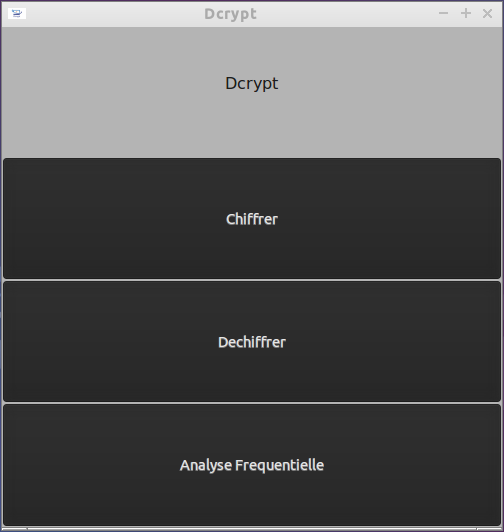
\includegraphics[scale=0.4]{1.png}\end{center}
			
			
			
	\section{Menu Cryptage}
		\begin{center}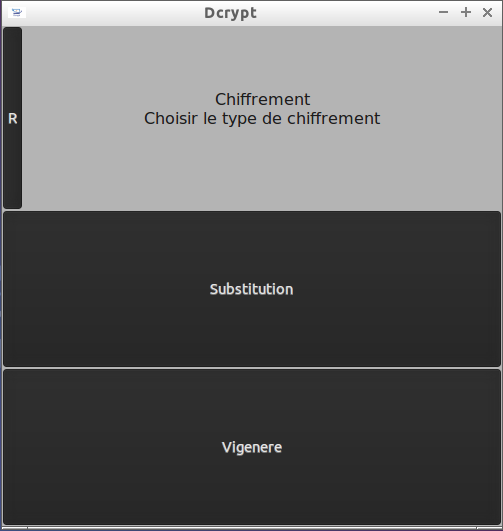
\includegraphics[scale=0.4]{2.png}\end{center}
		\subsection{Cryptage Substitution}
			\begin{center}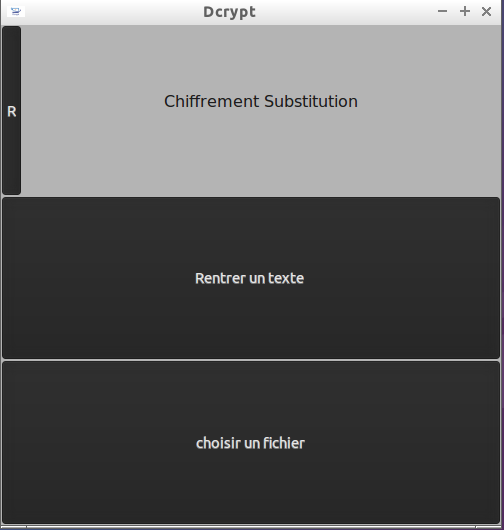
\includegraphics[scale=0.4]{3.png}\end{center}
			resultat\\
			\begin{center}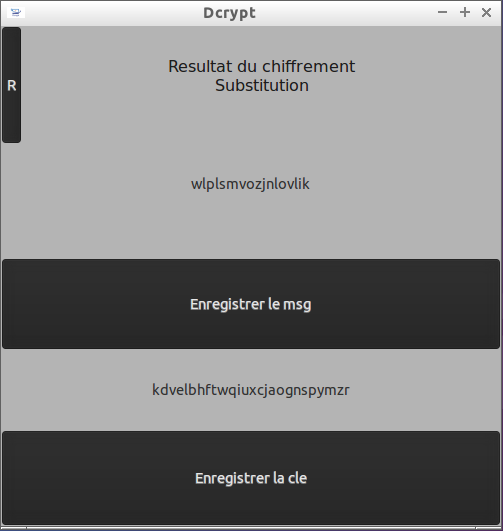
\includegraphics[scale=0.4]{5.png}\end{center}
		\subsection{Cryptage Vigenere}
			\begin{center}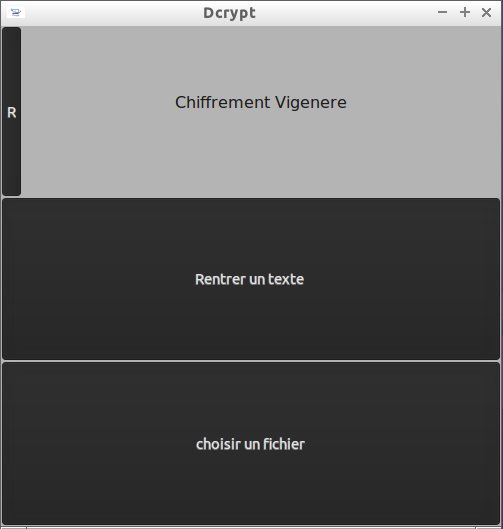
\includegraphics[scale=0.4]{6.png}\end{center}
			\begin{center}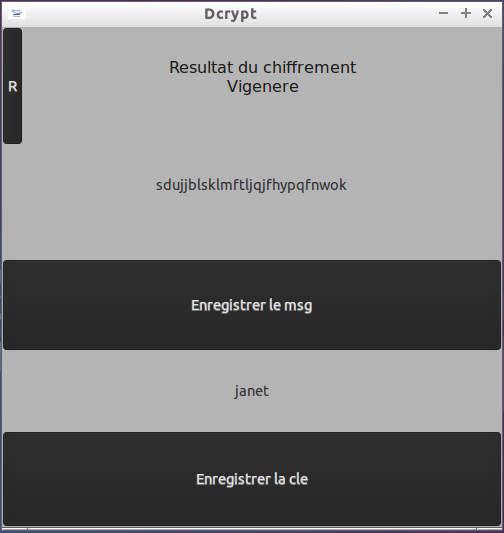
\includegraphics[scale=0.4]{7.png}\end{center}
		
		
	\section{Menu Decryptage}
		\begin{center}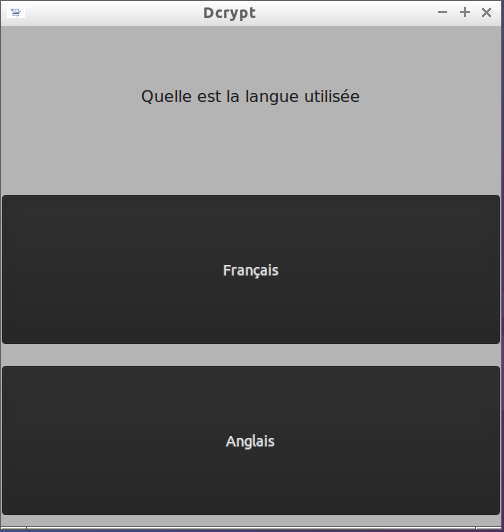
\includegraphics[scale=0.4]{8.png}\end{center}
		\begin{center}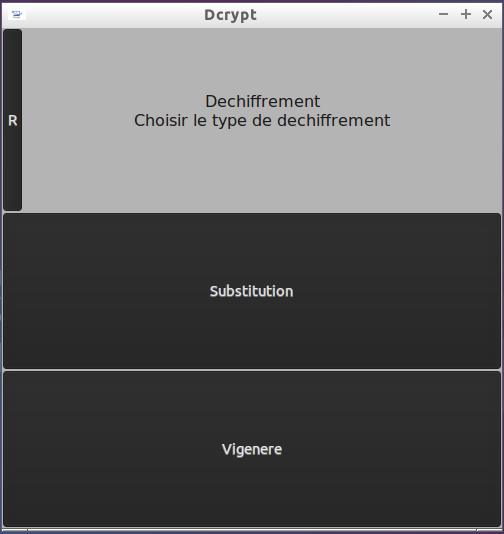
\includegraphics[scale=0.4]{9.png}\end{center}
		\subsection{Deryptage Substitution}
			\begin{center}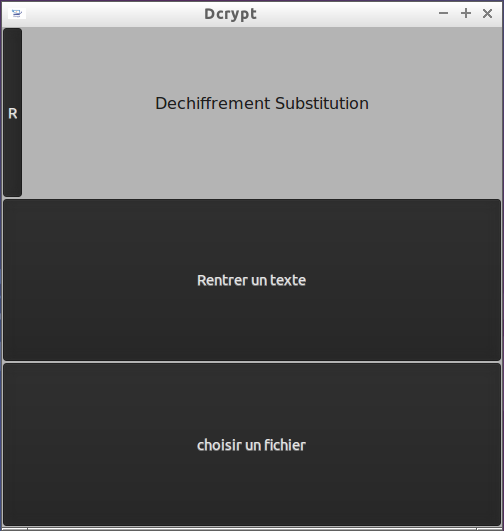
\includegraphics[scale=0.4]{10.png}\end{center}
			\begin{center}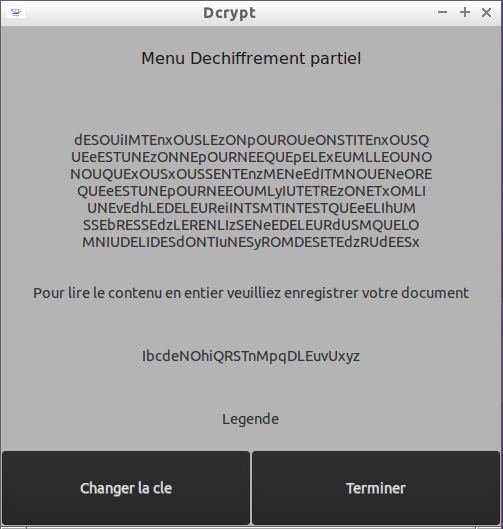
\includegraphics[scale=0.4]{13.png}\end{center}
			\begin{center}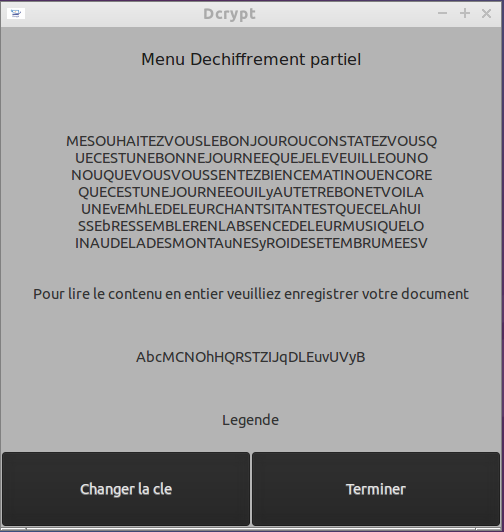
\includegraphics[scale=0.4]{11.png}\end{center}
			\begin{center}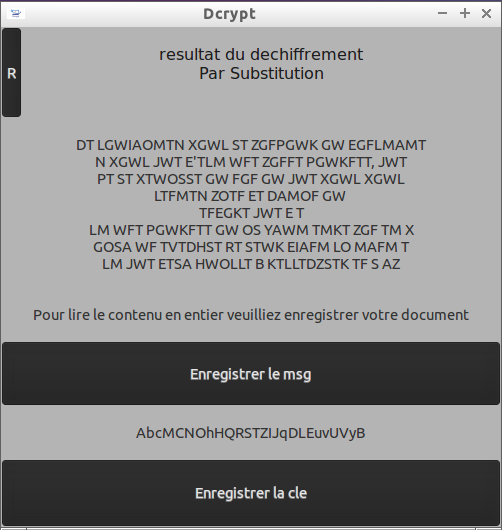
\includegraphics[scale=0.4]{12.png}\end{center}
		\subsection{Decryptage Vigenere}
			\begin{center}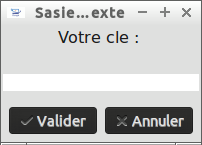
\includegraphics[scale=0.4]{22.png}\end{center}
			\begin{center}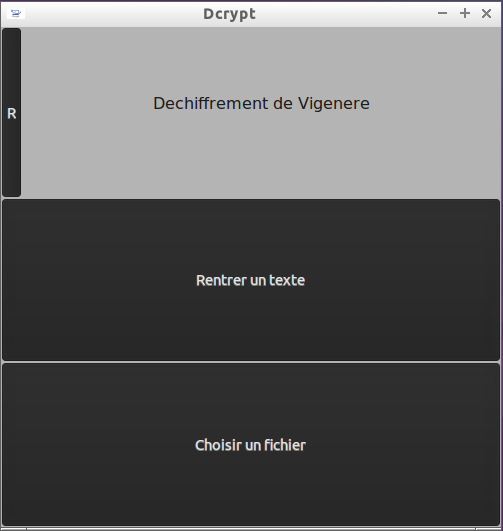
\includegraphics[scale=0.4]{14.png}\end{center}
			\begin{center}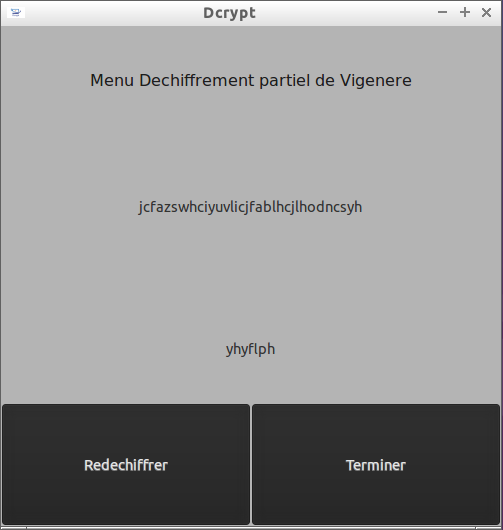
\includegraphics[scale=0.4]{15.png}\end{center}
			\begin{center}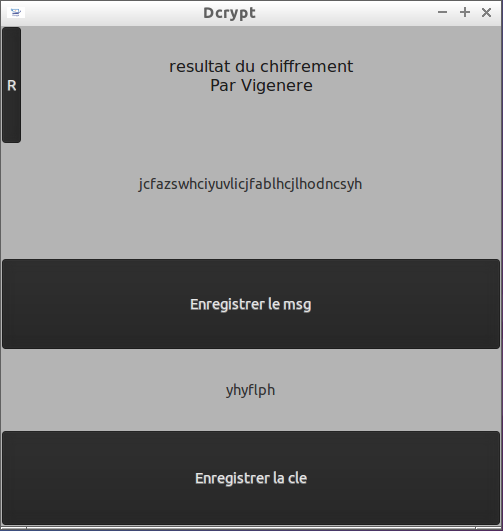
\includegraphics[scale=0.4]{16.png}\end{center}
		
		
	\section{Menu Analyse Frequentielle}
		\begin{center}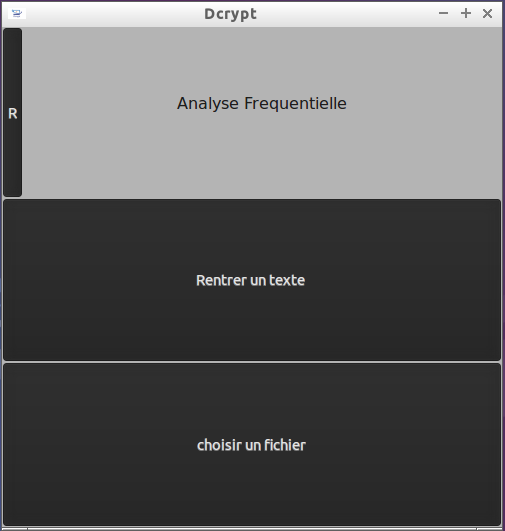
\includegraphics[scale=0.4]{17.png}\end{center}
		\begin{center}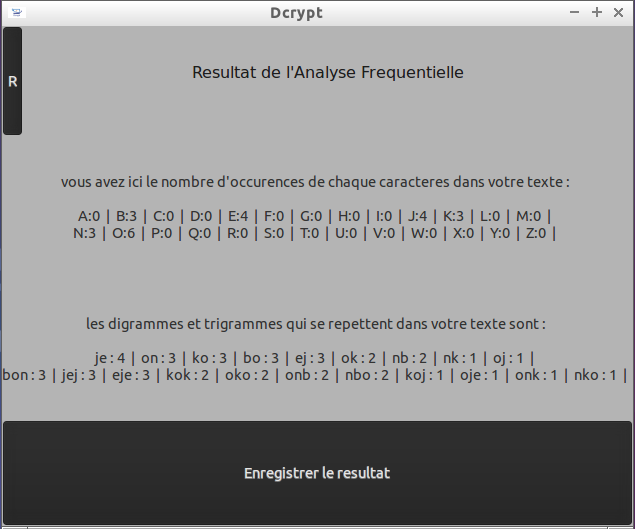
\includegraphics[scale=0.4]{18.png}\end{center}
	\section{entrer un texte}
		\begin{center}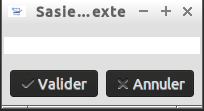
\includegraphics[scale=0.4]{21.png}\end{center}
	\section{les chargements/enregistrement de fichiers}
		\begin{center}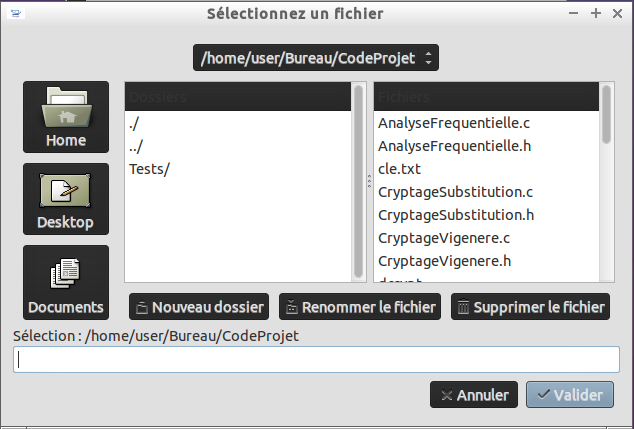
\includegraphics[scale=0.4]{19.png}\end{center}
		\begin{center}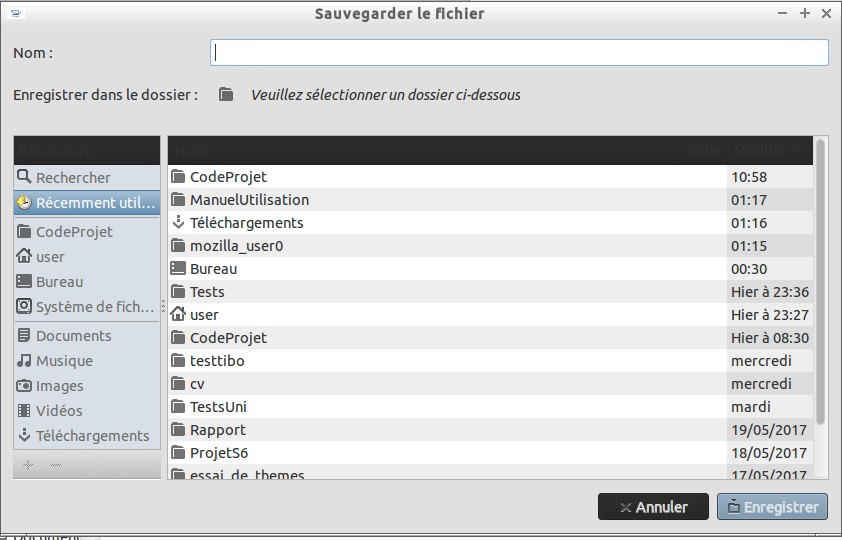
\includegraphics[scale=0.4]{20.png}\end{center}
\end{document}
